With the background of the high-level foundations presented in chapter~\ref{chap:design}, this chapter details the underlying implementation of the modules of the whole system. All source code has been written in JavaScript. \texttt{DHT} is run as a Node.js server and \texttt{Shuttle} runs as a client-side web application. Rymd is the platform independent core module containing the business logic of the system. All other modules contain the specific implementations for each problem area (see figure~\ref{fig:architecture}). Links to the source code for all modules are available in appendix~\ref{chap:source}.

In section~\ref{sec:modules} the overall areas of responsibility for the system modules were defined. This resulted in the following concrete modules described in this chapter:

\begin{description}
  \item[Rymd] The business logic for the system. Has references to the other modules through dependency injection.
  \item[Shuttle] The front-end prototype – a client-side web application.
  \item[DHT Client] Module which looks up records in the Namecoin blockchain through a NodeJS web service (see appendix~\ref{chap:source}).
  \item[RymdCrypto] Module for cryptography.
  \item[IndexedDBStore] Module for data and key storage.
  \item[PeerJS Connection] Module for communication with the PeerJS service.
\end{description}

\begin{figure}[ht]
\centering
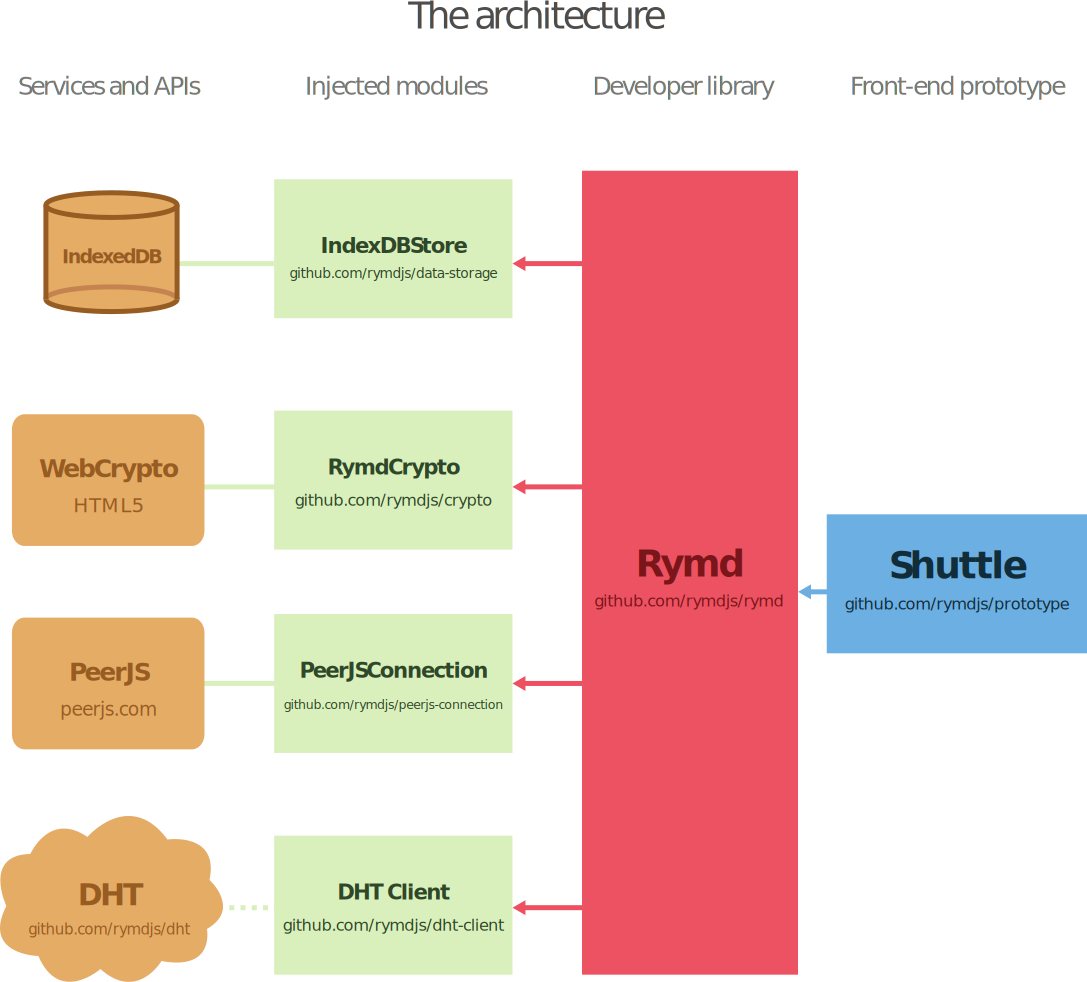
\includegraphics[width=\textwidth,height=0.4\paperheight,keepaspectratio
]{figures/architecture}
\caption{The modules and external APIs utilized in Rymd and Shuttle}
\label{fig:architecture}
\end{figure}

\section{Rymd}
\label{sec:rymd}

The Rymd library is the only truly implementation-agnostic module and should be runnable on any platform as long as implementation modules are dependency injected. It defines the business logic for behaviour such as:

\begin{itemize}
  \item The structure of resources and metadata
  \item The communication and authentication flow
  \item The \emph{resource store}: How resources are saved and identified independent of implementation
  \item Management of cryptographic keys
  \item Session management
\end{itemize}

Applications utilizing Rymd will generally instantiate a \texttt{RymdNode} object, which is the main entry point of the library and inject implementation modules. The RymdNode object will then act as the interface between the application and the Rymd library. The public interface of \texttt{RymdNode} is listed in listing~\ref{lst:rymdnode} along with the method signatures and return values.

\begin{Code}
\begin{lstlisting}[caption={Public methods of \texttt{RymdNode}}, label={lst:rymdnode}]
// Method signatures on the form <name>: [(<parameter>:<type> ...)]:<Return type>

// Initialize network and connection handlers from an identity
init: (identity:String):Promise

// If the RymdNode is initialized with an identity or not.
isAlive:Boolean

// Set the private key for an identity
setPrivateKey: (key:Key, identity:String):Promise(guid)

// Get the private key for an identity
getPrivateKey: (identity:String):Promise(key)

// Get the public key for an identity
getPublicKey: (identity:String):Promise(key)

// Get the RymdNode's current identity name
currentIdentity:String

// Connect to another identity (RymdNode)
connect: (identity:String):Promise(connection)

// Share a resource with a guid with another identity
shareResource: (guid:String, identity:String):Promise

// Request (download) a shared resource with a guid
requestResource: (guid:String):Promise

// Destroy a resource with a guid
destroyResource: (guid:String):Promise
\end{lstlisting}
\end{Code}

\texttt{RymdNode} triggers certain events on itself, which can be used for handling incoming resource sharing proposals, resource download requests, and more. The complete list of events are listed in listing~\ref{lst:rymdnode_events}. These events might initially be triggered inside some injected module, but \texttt{RymdNode} listens to events and triggers them on itself in order to present a coherent external event interface. For instance, the \texttt{request} event is triggered inside the PeerJS Connection module (section~\ref{sec:p2p}) and bubbled up to \texttt{RymdNode}.

\begin{Code}
\begin{lstlisting}[caption={Events triggered on \texttt{RymdNode}}, label={lst:rymdnode_events}]
App.rymdNode.on('init', function(identity) {
  // This RymdNode is finished initializing with a given 'identity'
});

App.rymdNode.on('resource', function(peerName, resource) {
  // Incoming resource from 'peerName'
});

App.rymdNode.on('request', function(peerName, data, connection) {
  // Incoming request for a resource (whose metadata are in 'data') from 'peerName'
});

App.rymdNode.on('share', function(peerName, data, connection) {
  // Incoming share request from 'peerName' with resource metadata in 'data'
});
\end{lstlisting}
\end{Code}

\section{Shuttle}
\label{sec:shuttle}
The front-end prototype was built in order to test and implement the features of Rymd. Early versions included a minimum viable interface for adding, showing and sending files. This was further iterated over, ending up letting the user:

\begin{itemize}
  \item Add files through form control or drag-and-drop
  \item Share, view and delete files
  \item Login (verifies with the DHT, see~\ref{sec:authentication})
  \item Get in-app notifications for incoming sharing requests
  \item Download remote files that have been shared by other users
  \item Add custom encryption keys
\end{itemize}

Shuttle uses Rymd's functionality by instantiating a global \texttt{RymdNode} object (see~\ref{sec:rymd}). This effectively makes Shuttle a node in the network. In-app notifications are shown by listening to certain events on the \texttt{rymdNode} object. Shuttle uses \texttt{RymdNode's} external interface in order to control the application logic, such as responding to and initiating resource sharing requests (see listings~\ref{lst:shuttle_request} and \ref{shuttle_show_file}).

\begin{Code}
\begin{lstlisting}[caption={Incoming download request}, label={lst:shuttle_request}]
// Listen to incoming request events and immediately send the wanted resource
App.rymdNode.on('request', function(peer, data, connection) {
  // Access the rymdNode object's resource store
  App.rymdNode.store.getResource(data.guid, true)
    .then(connection.sendResource.bind(connection));
});
\end{lstlisting}
\end{Code}

\begin{Code}
\begin{lstlisting}[caption={Show a downloaded file}, label={lst:shuttle_show_file}]
var guid = <guid fetched from the application interface>;

App.rymdNode.store.getDecryptedResource(guid).then(function(resource) {
  // Create URL to file with correct MIME type and show in new window
  var objectUrl = Rymd.Utils.toObjectURL(resource.data.data, resource.metadata.type);
  window.open(objectUrl, "_blank");
});
\end{lstlisting}
\end{Code}

\section{Authentication (DHT, DHT Client)}
\label{sec:authentication}
Since the default authentication implementation utilizes Namecoin, which can not be accessed directly from a web application, a gateway service needs to be used. Therefore, the domain of authentication spans over several parts in separate systems:

\begin{description}
  \item[DHT] A NodeJS\footnote{http://nodejs.org} based server that looks up entries in the Namecoin blockchain. It is also used to keep track of session-based IDs, as described under~\ref{sec:communication}. This is the only module that runs outside of the Rymd library.
  \item[DHT-Client] Client-side interface module to the DHT.
  \item[ConnectionHandler] Submodule in the Rymd library. Implements the Needham-Schroeder-Lowe authentication business logic.
\end{description}

The idea with this separation is that the authentication algorithm is part of the core library, while derivative projects should be able to replace $DHT$ and $DHT-client$ with implementations using other stores such as Ethereum or Keybase without having to consider writing a secure authentication protocol, should they so desire.

\section{RymdCrypto}
\label{sec:cryptography}
The implementations of WebCrypto in Chromium supply key generation, but there is no support for persisting keys between sessions or even exporting private keys. W3C - the organization behind WebCrypto - have announced their intention to handle persistent key storage in an upcoming API called WebCrypto Key Discovery~\cite{WebCryptoKeyDiscovery:Online}. However, Google has no intention of implementing this in Chromium before the WebCrypto API is finalized. WebCrypto Key Discovery API was originally intended to be a part of the WebCrypto API but was extracted in order to decrease implementation complexity.

\subsection{Algorithms}
Since Rymd uses asymmetric keys for authentication, RymdCrypto should supply asymmetric signing and encryption schemes using the same keys. Considering the support in WebCrypto, this leaves RSA based schemes as the only alternatives (See table~\ref{table:webcryptoapi}). There are only two RSA based encryption schemes that are part of WebCrypto: $RSAES-PKCS1-v1.5$ and $RSA-OAEP$. $RSAES-PKCS1-v1.5$ is currently the only one that is implemented in Google Chrome, and is therefore the current choice for Rymd.  Rymd uses $RSASSA-PKCS1-v1.5$ for signing, mainly because it is recommended by the working group behind the WebCrypto API.

For encryption of resources, a symmetric algorithm is used. AES-CBC is a fast and simple to use symmetric key algorithm based on AES using cipher block chaining~\cite{AESISFAST:Online}.

Finally, a good hashing algorithm is needed in order to avoid collision of hashes, in other words to avoid having two generated hash values being exactly the same (similar to the \emph{birthday problem}~\footnote{http://statistics.about.com/od/ProbHelpandTutorials/a/What-Is-The-Birthday-Problem.htm}). For hashing purposes RymdCrypto uses SHA-256 as explained in section~\ref{sec:creationofresources}.


%Cryptoback.js
% \begin{Code}
% \begin{lstlisting}[caption={Included database operations}, label={lst:cryptoback}]
%  //dependecies cryptoback.js
%   var rsa = require('bignumber-jt'),
%       Q = require('q');

%  //dependecies crypto.js
%   var root = this,
%     Q = require('q'),
%     cryptojs = require('crypto-js'),
%     utils = require("./cryptoback");
% \end{lstlisting}
% \end{Code}

% add text about hashing
% why is the hashing in
\begin{table}[ht]
\centering
\begin{tabular}{lcccccc}
Algorithm name & Type & Encrypt & Decrypt & Sign & Verify & ImportKey \\
RSAES-PKCS1-v1\_5 & ASYM & x & x &  &  & x \\
RSASSA-PKCS1-v1\_5 & ASYM &  &  & x & x & x \\
RSA-PSS & ASYM &  &  & x & x & x \\
RSA-OAEP & ASYM & x & x &  &  & x \\
ECDSA & ASYM &  &  & x & x & x \\
AES-CTR & SYM & x & x &  &  & x \\
AES-CBC & SYM & x & x &  &  & x \\
AES-CMAC & SYM &  &  & x & x & x \\
AES-GCM & SYM & x & x &  &  & x \\
AES-CFB & SYM & x & x &  &  & x
\end{tabular}
\caption{Some WebCrypto API algorithms}
\label{table:webcryptoapi}
\end{table}

Commercial RSA certificates are more widely deployed compared to DSA certificates. Furthermore, the asymmetric keys are wrapped in PKCS\#8 and SPKI certificates while the symmetric key exist in raw format. \emph{The Private-Key Information Syntax Standard} (PKCS\#8) defines a way to store the private key, and the \emph{Simple Public Key Infrastructure} (SPKI) defines a way to store the public key. All three standards was chosen because they are the only three formats that is currently supported by Chromium~\cite{ImplementedChromium:Online}.

\subsection{Libraries}
Until the WebCrypto Key Discovery API is available, the RymdCrypto module generates pseudo-random keys through the external library \emph{bignumber-jt}\footnote{https://www.npmjs.org/package/bignumber-jt}. To do low-level key generation directly in JavaScript is bad practice and is performed in order to make Rymd runnable until a more solid solution is available.

Furthermore, IndexedDB is used as makeshift storage since the WebCrypto API lacks functionality for storing keys between sessions, or even exporting private keys. In order to use IndexedDB for the keys they need to be parsed to certificates. This is also handled by bignumber-jt. All certificates have a static key size where asymmetric keys are of 1024 bits and symmetric keys are of 256 bits. Key parsing and generation is currently handled by bignumber-jt.

Hashing is handled by the external library \emph{crypto-js}\footnote{https://github.com/evanvosberg/crypto-js}.

\subsection{Interface}

The RymdCrypto library exposes functions handling key generation, encryption, decryption, signing, verification, and hashing. The methods and their signatures are presented in listing~\ref{lst:cryptointerface}.

\begin{Code}
\begin{lstlisting}[caption={Public methods of \texttt{RymdCrypto}}, label={lst:cryptointerface}]
// Method signatures on the form <name>: [(<parameter>:<type> ...)]:<Return type>


// Generate symmetric key 
generateSymmetric: ():Promise(key)

// Generate asymmetric key pair 
generateKeyPair: ():Promise(privateKey, publicKey)

// Import key. purpose: encrypt|sign. type: public|private|secret
importKey: (type:String, purpose:String, key:Uint8Array):Promise(key)

// Export key
exportKey: (WebCrypto::Key key):Promise(key)

// Decrypt data with key
decryptData: (WebCrypto::Key key, Uint8Array data):Promise(Uint8Array data)
decryptBlob: (WebCrypto::Key key, Blob blob):Promise(Uint8Array data)

// Encrypt data with key
encryptData: (WebCrypto::Key key, Uint8Array data):Promise(Uint8Array data) 
encryptBlob: (WebCrypto::Key key, Blob blob):Promise(Uint8Array data) 

// Sign data using asymmetric key
signKey: (WebCrypto::Key key, Uint8Array data):Promise(Uint8Array signature)

// Verify data signed using asymmetric key.
verifyKey: (WebCrypto::Key key, Uint8Array data, Uint8Array signature):Promise(Boolean result)

// Hashes data.
hashString: (String data):Promise(String hash)
hashBlob: (Blob blob):Promise(String hash)


\end{lstlisting}
\end{Code}
% before it's imported into its low-level interface.
% \begin{Code}
% \begin{lstlisting}[caption={Common database operations}, label={lst:cryptointerface}]
% generateKeyPair: function() -> Promise({Uint8array,Uint8array})
% exportKey: function(WebCrypto::Key) -> Promise({Uint8array})
% importKey: function(String,Uint8array) -> Promise(WebCrypto::Key)
% signKey: function(WebCrypto::Key,Uint8Array) -> Promise
% verifyKey: function(WebCrypto::Key,Uint8Array,Uint8Array) -> Promise
% encrypt**: function(WebCrypto::Key,Uint8Array??) -> Promise(Arraybuffer)
% decrypt**: function(WebCrypto::Key,Uint8Array??) -> Promise(Arraybuffer)
% hash**: function(blob)  -> Promise(blob)
% generateSymmetricKey: function() -> Promise(WebCrypto::Key)
% \end{lstlisting}
% \end{Code}


\section{IndexedDBStore}
\label{sec:indexeddbstore}

The main task for the data storage module was to abstract away the low-level methods in IndexedDB (the backing store used, see section~\ref{sec:indexeddb}). An API example can be found in listing~\ref{lst:indexeddbapi}. The module supports use of multiple object stores and auto-generation of GUID keys.

\begin{Code}
\begin{lstlisting}[caption={Common database operations}, label={lst:indexeddbapi}]
var IndexedDbStore = require('indexeddbstore')

var Store = new IndexedDbStore('myStore')

// Fetch all records as an array
Store.all().then(function(records) { ... })

// Create a record
Store.create('A record').then(function(record){ ... })

// Insert a record
Store.save('A record').then(function(guid){ ... })

// Fetch a record by GUID
Store.get(guid).then(function(record) { ... })

// Delete a record by GUID
Store.destroy(guid).then(function(record) { ... })
\end{lstlisting}
\end{Code}

The largest challenge came to the edge cases when storing files, or as they are called in web browser: \emph{Blobs}. Since at present only Firefox can store blobs directly in IndexedDB, an alternate route had to be taken for other browsers. Initially the module used conditionals and converted incoming data to and from \emph{ArrayBuffers} (the browser construct for raw byte streams). But since ArrayBuffers are just the raw data, all metadata for the blobs (such as filename, timestamps, size) would be lost when saving as an ArrayBuffer. In early versions of the data storage module this metadata would be stored in a separate store in the database, but this was too tightly coupled and was removed. The final implementation is storing data as-is – any metadata must be saved explicitly in a separate operation.

The asynchronous API of IndexedDB is relatively verbose and complex. It makes heavy use of event driven programming and thus the developer communicates with the database with callbacks. By the use of \emph{Promises}~\cite{Promises:Online}, the asynchronous, callback-based methods in the IndexedDB API was made streamlined and simple to manage.

\section{PeerJS Connection}
\label{sec:p2p}

Rymd leverages the open source project PeerJS\footnote{http://peerjs.com}, which simplifies sending peer-to-peer data between clients. This module was therefore constructed, in line with the project guidelines regarding modularity, to contain PeerJS-specific code and to provide an independent interface which does not reveal the details of PeerJS's inner workings. If changes in Rymd's requirements makes the choice of PeerJS obsolete, then the changes will be isolated and one should still be able to depend on the same interface.

PeerJS utilizes WebRTC and is essentially split into two components: a server which acts as the signaling channel, and a client-side API which interacts with the server as well as other peers. The server only handles the brokering of connections, which implies that only the data necessary for negotiating a connection is sent through this point. For communication between the server and the clients, that is the signaling protocol, PeerJS utilizes both WebSockets and XMLHttpRequest~\cite{PeerjsGithub:2014:Online}. After a connection has been setup between two clients, the server is no longer needed in order for them to communicate.

% - explain how peer.js works.
The following steps explain how PeerJS brokers connections:
\begin{enumerate}
\item Two clients connect to the PeerJS server, using the client-side API.
\item The server returns unique IDs for each of the clients.
\item One of the clients connects to the other using the client-side API, where the unique ID for the other one is provided. The PeerJS server then forwards the information needed to set up a peer-to-peer connection to the other client.
\end{enumerate}

In order to map the identity registered in the Namecoin blockchain to the ID supplied by the PeerJS server, the DHT service is used. After a client has connected to a PeerJS server, it supplies the data regarding the server IP and the generated ID to the DHT. When another client wants to create a peer-to-peer connection, it queries the DHT service for the Namecoin identity, which then returns the IP for the PeerJS server and the ID for the client.

To ensure the integrity of users it is vital that the communication with the PeerJS server and the DHT service is encrypted. The current implementation utilize the WebSocket protocol and the XHR API, which are not encrypted per default, for communication over these channels. Therefore an implementation running on top of the SSL/TLS protocol has to be in place before the project can be considered to have reached a releasable state.

\clearpage

\section{Testing}
\label{sec:testing}

Automatic unit tests have been implemented where possible. Thanks to the use of isolated modules test suites were able to be short and concise. Mocha was used as test runner, with Chai as assertion library (please see appendice~\ref{chap:libraries} for links to external libraries used). Listing~\ref{lst:testsuite} shows an excerpt from the test suite, where simple operations are tested and their results are verified.

\begin{Code}
\begin{lstlisting}[caption={Sample test suite}, label={lst:testsuite}]
describe('IndexedDBStore', function() {

  var db;

  beforeEach(function() {
  	db = new IndexedDBStore({
  		dbName: 'test'
  	});
  });

  it('should have a database name', function() {
  	db.name.should.equal('test');
  });

  it('should save a record and return an id', function() {
  	return db.save({foo: 'bar'})
  	.then(function(id) {
  		id.should.be.a('String');
  	});
  });

  it('should retrieve a given record', function() {
  	return db.save({foo: 'bar'})
      .then(db.get.bind(db))
      .then(function(record) {

  		record.should.be.an('Object');
  		record.data.foo.should.equal('bar');
  	});
  });
});
\end{lstlisting}
\end{Code}

No integration or functional tests have been written for testing larger parts of the system. This is due to the fast iteration of the library's interface and constant change in implementation.
